\documentclass[12pt]{article}
\usepackage[utf8]{inputenc}
\usepackage[T1]{fontenc}
\usepackage[brazil]{babel}
\usepackage[useregional=numeric]{datetime2}
\usepackage{array}
\usepackage{graphicx}
\usepackage{float}
\usepackage{hyperref}

% Caminho para diretório das imagens
\graphicspath{{./images/}}

% Configuração dos hyperlinks
\hypersetup{
    colorlinks=true,
    linkcolor=black,
    filecolor=magenta,
    urlcolor=blue,
}

\title{
    PyRingo - Especificações de Requisitos
    %% Gambiarra para mostrar "código do documento"
    \\REQ\_PR\_JogoRingo\_2021Fev19
}
\author{Gabriel Carneiro\\Lorenzo Maturano\\Luiz Gustavo Saibro\\
% Gambiarra para mostrar versão do documento na capa
v1.4}
\date{\today}

\begin{document}

% Logo da UFSC
\begin{figure}
    
\includegraphics[scale=0.3]{logo-ufsc}
    \centering
    \label{fig:logo-ufsc}
\end{figure}

% Titulo referenciando as informações listadas da linhas 7 a 9
\maketitle

\newpage

% * -> Sessão não numerada
\section*{Tabela de Versionamento}

% Tabela de versões
% \\ -> Quebra de linha na tabela
% & -> Separa as colunas
% \hline -> Insere uma linha horizontal na tabela

\begin{center}
\begin{tabular}{|c|c|c|m{4.5cm}|}
    \hline
    Versão & Autor(es) & Data & Ação \\
    \hline
    1.0 & Gabriel Carneiro & 19/02/2021 & Construção do esqueleto da especificação de requisitos. \\
    \hline
    1.1 & Luiz Gustavo Saibro & 19/02/2021 &  Elaboração da especificação de requisitos\\
    \hline
    1.2 & Lorenzo Maturano & 25/02/2021 & Alterações no modelo do documento e elaboração da especificação de requisitos. \\
    \hline
    1.3 & Lorenzo Maturano & 25/03/2021 & Alterações de requisitos, conforme feedback do professor. \\
    \hline
    1.4 & Gabriel Carneiro & 09/05/2021 & Correções nas definições do jogo e melhoria nas descrições dos movimentos. \\
    \hline
\end{tabular}
\end{center}

\newpage

% Sumário gerado automaticamente
\tableofcontents

\newpage

\section{Introdução}
% Escreva aqui:

\subsection{Objetivo}
Desenvolvimento de um software \textbf{stand-alone}, modelando o jogo de tabuleiro e estratégia \textbf{Ringo}, na linguagem de programação \textbf{Python}.

\subsection{Definições}
% TODO: WIP
% Escreva aqui:
\textbf{Ringo} é um jogo de tabuleiro abstrato de estratégia e de dois jogadores.

\begin{itemize}
    \item \textbf{Argola}: componente do jogo, manipulado pelo jogador;
    \item \textbf{Peça}: componente do jogo, manipulado pelo jogador;
    \item \textbf{Posição}: local do tabuleiro que pode estar vazio, ocupado por uma peça, por um anel ou por uma peça e um anel;
%    \item \textbf{Argola Livre}: argola não ocupada por peça;
%    \item \textbf{Argola Ocupada}: argola ocupada por peça;
    \item \textbf{Posição Livre}: posição do tabuleiro não ocupada por argola ou peça;
    \item \textbf{Posição Ocupada}: posição do tabuleiro ocupada por argola ou peça;
\end{itemize}

O jogo é composto por \textbf{dois conjuntos de 10 peças e 4 argolas}, sendo cada conjunto com uma cor específica para identificar jogadores e um \textbf{tabuleiro} em formato de matriz, onde as peças do jogo são posicionadas.
\subsection{Referências}
\begin{itemize}
    \item \url{https://www.youtube.com/watch?v=V10gy_BnaNk}.
    \item \url{https://boardgamegeek.com/boardgame/261490/ringo/videos/all}.
    \item \url{https://www.youtube.com/watch?v=YHdRpfejvqQ&ab_channel=BoardGameGeek}.

\end{itemize}

\section{Regras do Jogo}
% Escreva aqui:

\subsection{Estado Inicial do Tabuleiro}

\begin{figure}[H]
    \centering
    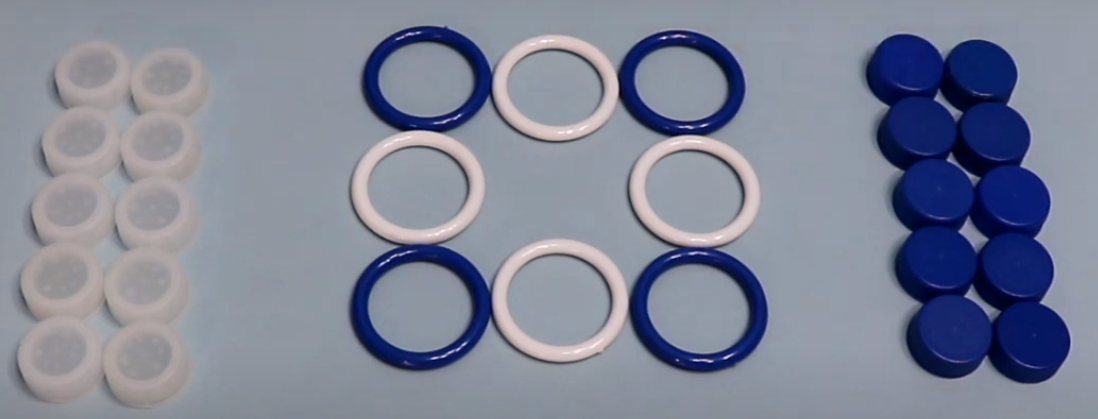
\includegraphics[width=0.75\textwidth]{ringo}
    \caption{Formação inicial do tabuleiro.}
    \label{fig:ringo}
\end{figure}

Um dos conjuntos de argolas ocupa as posições do canto, já o outro conjunto ocupa os espaços entre os cantos. Não é necessário manter o mesmo padrão de cores. Ou seja, em outra partida, os anéis brancos poderiam ocupar os cantos. As peças são inicialmente mantidos fora do tabuleiro.

\bigskip

\subsection{Objetivo}

Ganha o jogador que posicionar na vertical, na horizontal, ou na diagonal um conjunto de 4 peças ou 4 argolas consecutivos da sua cor.

\bigskip

\subsection{Movimentos}

Os movimentos podem ser divididos em dois momentos,
quando o jogador ainda possui peças e quando todas suas peças já estão em jogo

\begin{itemize}
    \item O jogador cujo o conjunto de argolas ocupam os cantos inicia o jogo.
    \item Se o jogador possui peças:

    \begin{itemize}
        \item O jogador executa duas ações por rodada: \textbf{movimentar peça e movimentar argola}.
        \item O jogador inicia colocando uma peça \textbf{dentro de alguma argola livre}, não importando a cor da argola.
        \item Após colocar sua peça a uma argola livre, o jogador deve movimentar a \textbf{argola que foi ocupada}.
        \item A argola pode ser posicionado em uma \textbf{posição livre}, de maneira adjacente a outra argola ou peça, podendo ser tanto na vertical quanto na horizontal.
    \end{itemize}
    \item Se todas peças estão em jogo:
    \begin{itemize}
        \item Agora, antes de colocar uma peça no tabuleiro, \textbf{o jogador deve remover uma de suas peças que foi colocada no tabuleiro}.
        \item Ao remover uma peça o jogador não pode segmentar o conjunto de peças e argolas em dois conjuntos separados.
    \end{itemize}
\end{itemize}


\section{Visão Geral do Sistema}

\subsection{Arquitetura do Software}
% Escreva aqui:
Software \textbf{stand-alone}, modelando o jogo \textbf{Ringo}, utilizando a linguagem de programação \textbf{Python} e o paradigma de \textbf{Programação Orientado a Objetos}.

\subsection{Premissas de Desenvolvimento}
% Escreva aqui:
\begin{itemize}
    \item Implementado em \textbf{Python}.
    \item Executável em qualquer ambiente com Python3.
    \item Script de instalação para criação de um ambiente virtual e instalação de dependências.
    \item Script de desinstalação.
    \item Interface gráfica.
    \item Modelagem UML utilizando o software \textbf{Visual Paradigm}.
\end{itemize}

\newpage

\section{Requisitos da Aplicação}
\subsection{Requisitos Funcionais}

\begin{itemize}
    \item \textbf{RF01 - Iniciar jogadores}: O programa deve possibilitar a criação de dois jogadores antes de iniciar um novo jogo, com seus respectivos nomes.
    \item \textbf{RF02 - Colocar peça na posição}: O programa deve possibilitar ao jogador inserir uma peça em seu turno em um local possível dentro das regras do jogo.
    \item \textbf{RF03 - Colocar argola na posição}: O programa deve possibilitar o jogador mudar a argola de posição em seu turno em um local possível, seguindo as regras do jogo.
    \item \textbf{RF04 - Remover peça de posição}: O programa deve possibilitar ao jogador remover uma peça de posição em seu turno em um local possível dentro das regras do jogo, quando não tiver mais peças disponíveis.
    \item \textbf{RF05 - Reiniciar partida}: O programa deve reiniciar a partida automaticamente após notificar o vencedor.
\end{itemize}

\subsection{Requisitos Não-Funcionais}
\begin{itemize}
    \item \textbf{RNF01}: O jogo deve ser desenvolvido utilizando a linguagem de programação Python, versão 3.
    \item \textbf{RNF02}: O jogo deve utilizar a biblioteca PyGame para desenvolver a interface gráfica.
    \item \textbf{RNF03}: O jogo deve ter uma única interface para os dois jogadores.
    \item \textbf{RNF04}: Para controle de versionamento utilizar o github.
\end{itemize}

\pagebreak

\section{Esboço da Interface Gráfica}
\begin{figure}[h]
    \centering
    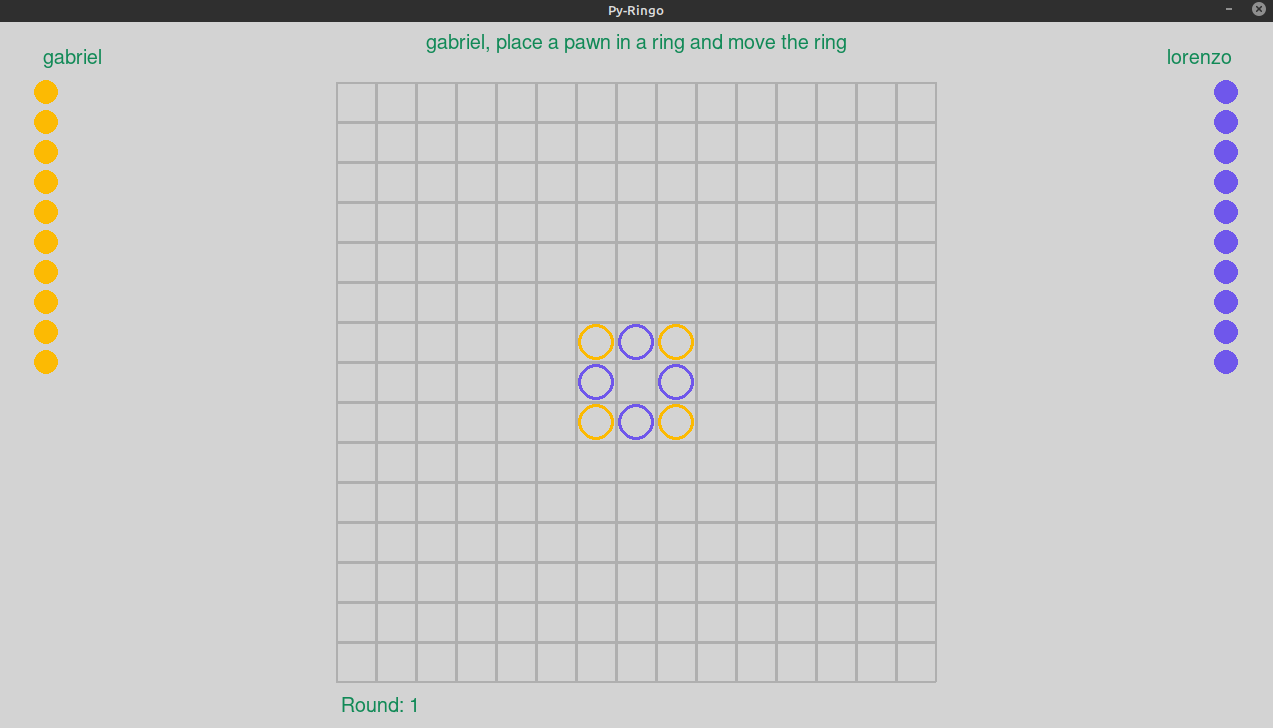
\includegraphics[scale=0.4]{interface}
    \caption{Esboço da Interface Gráfica}
    \label{fig:interface}
\end{figure}

\end{document}